% This file is part of BenchExec, a framework for reliable benchmarking:
% https://github.com/sosy-lab/benchexec
%
% SPDX-FileCopyrightText: 2007-2020 Dirk Beyer <https://www.sosy-lab.org>
%
% SPDX-License-Identifier: Apache-2.0

\documentclass[tikz, border=3mm, convert=pdf2svg]{standalone}
\usetikzlibrary{arrows}
\usetikzlibrary{calc}
\usetikzlibrary{fit}
\usetikzlibrary{positioning}

\begin{document}
  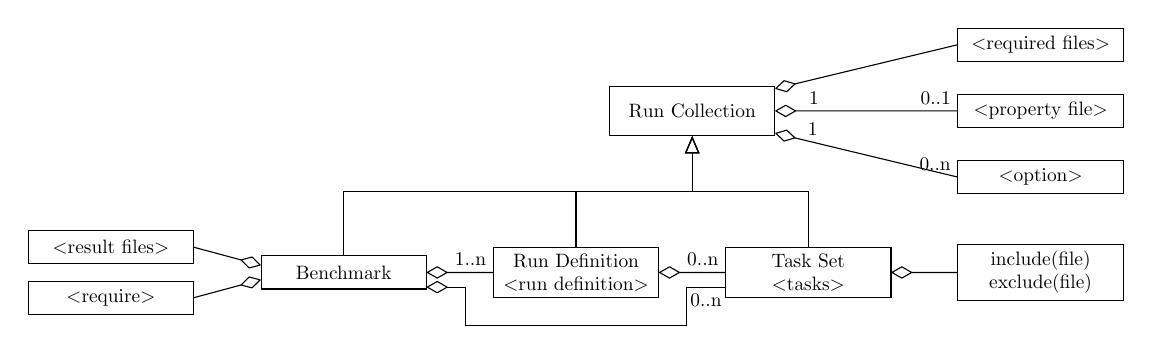
\begin{tikzpicture} [
        scale = 0.7,
        transform shape,
        node distance = 1.2cm,
        every node/.style = {
          align = center,
          %font = \footnotesize,
        },
        umlbox/.style = {
          draw,
          minimum width = 3cm,
          minimum height = 0.6cm,          
        },
        inherit/.style = {
          draw,
          -open triangle 45,
        },
        aggregation/.style = {
          draw,
          open diamond-,
        },
        cust-fit/.style={%
          % draw,
          inner sep = 0pt,
          transform shape = false,
        }
      ]

    % textboxes
    \node [umlbox] (resFiles) {$<$result files$>$};
    \node [umlbox, below = 0.3cm of resFiles] (require) {$<$require$>$};
    \node [fit={(resFiles) (require)}, cust-fit] (fitBox) {}; 

    \node [umlbox, right = of fitBox] (benchmark) {Benchmark};

    \node [umlbox, right = of benchmark] (runDef) {Run Definition\\$<$run definition$>$};
    \node [umlbox, right = of runDef] (taskSet) {Task Set\\$<$tasks$>$};
    \node [fit={(runDef) (taskSet)}, cust-fit] (fitBox2) {}; 

    \node [umlbox, minimum height = 0.9cm, above = 2cm of fitBox2] (runCol) {Run Collection};

    \node [umlbox, right = of taskSet] (inclExcl) {include(file)\\exclude(file)};

    \coordinate (interectionPoint) at (runCol -| inclExcl);
    \node [umlbox, yshift = 1.2cm] at (interectionPoint) (reqFiles) {$<$required files$>$};
    \node [umlbox] at (interectionPoint) (propFile) {$<$property file$>$};
    \node [umlbox, yshift = -1.2cm] at (interectionPoint) (opt) {$<$option$>$};
    %\node [umlbox, yshift = 1.2cm] at (interectionPoint) (reqFiles) {$<$required files$>$};
    %\node [umlbox, yshift = 0.4cm] at (interectionPoint) (inclFile) {$<$include file$>$};
    %\node [umlbox, yshift = -0.4cm] at (interectionPoint) (propFile) {$<$property file$>$};
    %\node [umlbox, yshift = -1.2cm] at (interectionPoint) (opt) {$<$option$>$};


    \draw[aggregation] (benchmark.175) -- (resFiles.east);
    \draw[aggregation] (benchmark.185) -- (require.east);
    \draw[aggregation] (benchmark.east) -- (runDef.west) coordinate [label=135:{1..n}];
    \draw[aggregation] (runDef.east) -- (taskSet.west) coordinate [label=135:{0..n}];

    \coordinate [below = 0.5cm of runDef] (dummyPoint);
    \draw[aggregation] (benchmark.350) -- ++(right:0.7cm) |- (dummyPoint);
    \draw (taskSet.190) to [edge label={0..n}] ++(left:0.7cm) |- (dummyPoint);

    \draw[inherit] (runDef) |- ($(runDef)!.5!(runCol)$) -| (runCol);
    \draw[inherit] (taskSet) |- ($(taskSet)!.5!(runCol)$) -| (runCol);
    \draw[inherit] (benchmark) |- ($(benchmark)!.5!(runCol)$) -| (runCol);

    \draw[aggregation] (taskSet) -- (inclExcl);

    \draw[aggregation] (runCol.15) -- (reqFiles.west);
    \draw[aggregation] (runCol.east) to ++(right:0.7cm) coordinate [label=1] -- (propFile.west) coordinate [label=135:{0..1}];
    \draw[aggregation] (runCol.345) to ($(runCol.345)!0.7cm!(opt.west)$) coordinate [label=1] -- (opt.west) coordinate [label=135:{0..n}];
  \end{tikzpicture}
\end{document}
